\documentclass[12pt,a4paper]{article}
\XeTeXinputencoding "utf8"

\usepackage{fontspec}
\setmainfont{Times New Roman}

\usepackage{graphicx}

\graphicspath{{figures/}}
\setlength{\textwidth}{16.5cm}
\setlength{\oddsidemargin}{0.46cm}
\setlength{\textheight}{25.7cm}
\setlength{\topmargin}{-0.54cm}
\setlength{\headheight}{0pt}
\setlength{\headsep}{0pt}
\setlength{\parindent}{1.25cm}
\setlength{\parskip}{0pt}
\linespread{1.25}
\emergencystretch=3em
\renewcommand{\contentsname}{Содержание}
\renewcommand{\tablename}{Таблица}
\renewcommand{\figurename}{Рисунок}

\begin{document}

\begin{titlepage}
    \begin{center}
        \textbf{Белорусский государственный университет}\\\relax
        ФМиИС, ФПМИ\\[0.5cm]

        \vfill

        {\large Лабораторная работа № 2}\\[0.5cm]
        {\Large\textbf{Обработка полутоновых изображений}}\\[0.3cm]
        {\large Вариант 4}

        \vfill
    \end{center}

    \begin{flushright}
        Выполнил: студент группы 4\\\relax
        Герасимович Данила Александрович\\
    \end{flushright}

    \vfill

    \begin{center}
        [Город]\\
        2026
    \end{center}
\end{titlepage}

\tableofcontents
\clearpage

\section{Цель работы}

Изучить методы повышения контраста полутоновых изображений и методы
обнаружения точек, линий и перепадов яркости. Реализовать эти методы в
приложении с графическим интерфейсом, проверить их на исходном и изменённых
тестовых изображениях и сравнить результаты.

\section{Постановка задачи}

Согласно заданию для варианта 4 необходимо реализовать линейное
контрастирование и эквализацию гистограммы, а также сегментацию изображения
по точкам, линиям и перепадам яркости. Приложение должно предоставлять
графический интерфейс и набор тестовых изображений, в том числе
малоконтрастное, зашумленное и размытое.

\section{Теоретические сведения}

\subsection{Линейное контрастирование}

Пусть $I(x,y)$ --- яркость пикселя исходного изображения, а $I_{\min}$ и
$I_{\max}$ --- минимальная и максимальная яркости изображения. Линейное
растяжение диапазона задаётся формулой
\[
    I_s(x,y) =
    255\frac{I(x,y)-I_{\min}}{I_{\max}-I_{\min}},
    \qquad I_{\max}>I_{\min}.
\]
Результат ограничивается диапазоном $[0,255]$ и сохраняется как 8-битное
изображение. При постоянной яркости результат заполняется нулями.
Преобразование использует весь доступный диапазон яркости, но не
перераспределяет частоты отдельных уровней.

\subsection{Эквализация гистограммы}

Гистограмма $h(k)$ показывает число пикселей яркости $k$, где
$k\in\{0,\ldots,255\}$. По ней вычисляется функция распределения
\[
    C(k)=\sum_{j=0}^{k}h(j).
\]
Эквализация отображает уровни яркости на основе нормированной накопленной
гистограммы. В общем виде преобразование можно записать как
\[
    I_e(x,y) =
    \mathrm{round}\left(
        \frac{C(I(x,y))-C_{\min}}{MN-C_{\min}}\cdot255
    \right),
\]
где $M\times N$ --- размер изображения, а $C_{\min}$ --- первое ненулевое
значение накопленной гистограммы. На практике в программе преобразование
выполняет функция \texttt{equalizeHist} библиотеки OpenCV.

\subsection{Обнаружение точек}

Лапласиан является второй производной изображения и реагирует на резкие
локальные изменения яркости. В программе вычисляется дискретный лапласиан
с ядром размера $3\times3$, после чего используется модуль отклика
$R(x,y)=|\nabla^2 I(x,y)|$. Точка отмечается, если отклик превышает порог
\[
    T=\max\bigl(30,\; P_{99.5}(R)\bigr),
\]
где $P_{99.5}$ --- 99,5-й процентиль значений отклика. Выбор процентильного
порога ограничивает число наиболее сильных откликов, помечаемых как точки.

\subsection{Обнаружение линий}

Для поиска линий сначала применяется гауссово сглаживание и детектор
границ Кэнни. Затем к границам применяется вероятностное преобразование
Хафа. В пространстве параметров прямая задаётся уравнением
\[
    \rho=x\cos\theta+y\sin\theta.
\]
Программа отображает найденные отрезки поверх исходного изображения.
Минимальная длина отрезка и порог накопителя задаются на основе меньшей
стороны изображения; небольшой допустимый разрыв позволяет объединять
близкие фрагменты одной линии.

\subsection{Обнаружение перепадов яркости}

Операторы Собеля вычисляют приближённые производные $G_x$ и $G_y$ по
горизонтали и вертикали. Величина градиента оценивается как
\[
    G(x,y)=\sqrt{G_x(x,y)^2+G_y(x,y)^2}.
\]
В приложении нормированная величина градиента бинаризуется порогом 100.
Для сравнения также выводятся границы Кэнни, рассчитанные с порогами 50 и
150 после гауссова сглаживания изображения.

\section{Описание программы}

Программа написана на Python. Для чтения изображения и обработки используются
OpenCV и NumPy; графический интерфейс реализован средствами Tkinter, а
результаты и гистограммы выводятся средствами Matplotlib.

Главное окно позволяет выбрать тестовое изображение или загрузить собственный
файл. Для каждого выбранного изображения приложение одновременно показывает:
\begin{itemize}
    \item исходное изображение, min-max-контрастирование и эквализацию;
    \item результат обнаружения точек по лапласиану;
    \item отрезки, найденные преобразованием Хафа;
    \item бинаризованный градиент Собеля, границы Кэнни и величину градиента;
    \item гистограммы исходного, контрастированного и эквализированного
    изображений, а также нормированную CDF исходного изображения.
\end{itemize}

В набор тестов входят исходное изображение, малоконтрастная версия
$I_l=0.35I+80$, версия с аддитивным гауссовым шумом со среднеквадратичным
отклонением 20 и версия, сглаженная гауссовым фильтром $9\times9$.
Случайный шум генерируется с фиксированным начальным значением, поэтому
тестовые варианты воспроизводимы при повторном запуске. Загрузка файла
выполняется с преобразованием в градации серого.

\section{Эксперимент и результаты}

В качестве исходного тестового изображения использовано полутоновое
изображение размером $474\times843$ пикселя. Оно содержит небо, деревья,
траву и животных; на изображении присутствуют как плавные области, так и
мелкие детали и границы объектов.

\begin{figure}[!htbp]
    \centering
    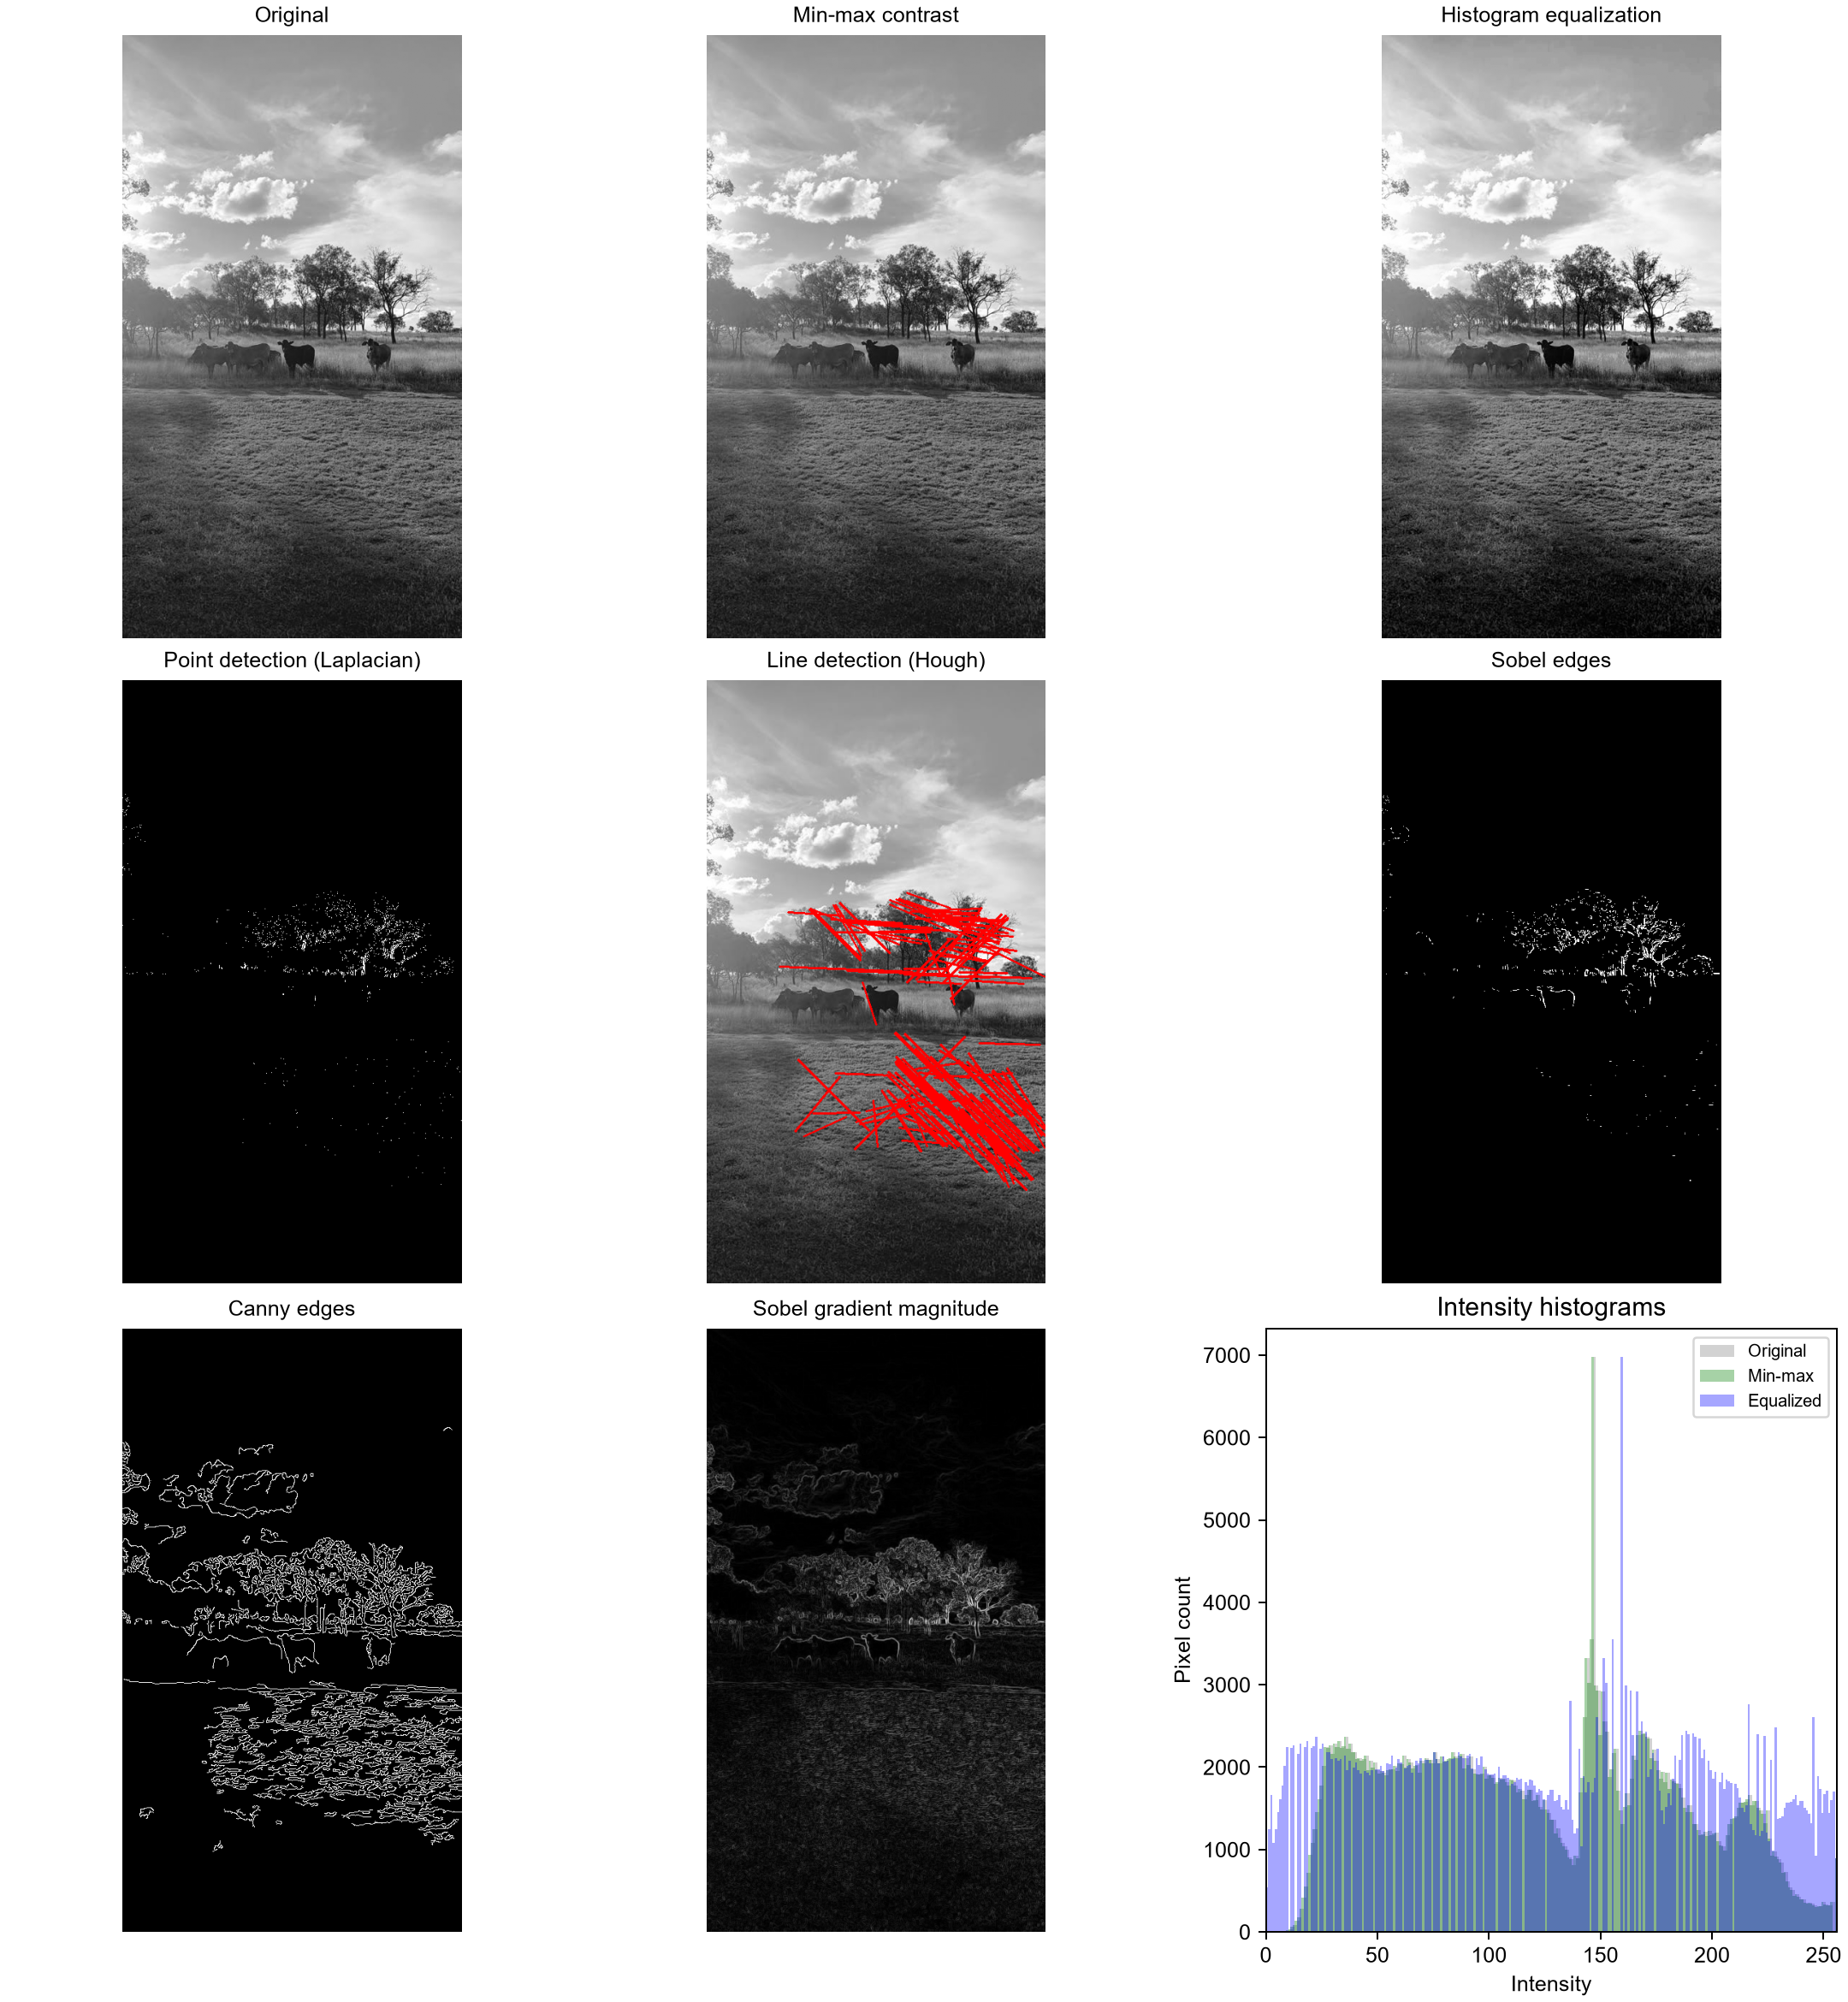
\includegraphics[width=\textwidth]{processing_results.png}
    \caption{Результаты обработки исходного тестового изображения}
    \label{fig:processing}
\end{figure}

На рисунке~\ref{fig:processing} представлены результаты всех методов.
Min-max-преобразование использует почти весь диапазон яркости. Эквализация
изменяет распределение уровней согласно CDF; визуально она усиливает
различия в ряде областей изображения. Отклик лапласиана выделяет небольшое
число сильных локальных деталей. Преобразование Хафа выделяет линейные
фрагменты на обнаруженных границах. Собель даёт бинарную карту сильных
градиентов, а Кэнни показывает более связные границы при выбранных порогах.

\begin{table}[!htbp]
    \centering
    \caption{Числовые характеристики преобразований}
    \label{tab:statistics}
    \begin{tabular}{|l|r|r|r|r|}
        \hline
        Изображение & Минимум & Максимум & Среднее & СКО\\
        \hline
        Исходное & 1 & 255 & 121{,}69 & 61{,}79\\
        Min-max & 0 & 255 & 120{,}70 & 61{,}80\\
        Эквализация & 0 & 255 & 128{,}13 & 73{,}60\\
        \hline
    \end{tabular}
\end{table}

В данном эксперименте стандартное отклонение после эквализации выросло
с 61{,}79 до 73{,}60, что согласуется с усилением контраста. Min-max
растяжение изменило границы диапазона с $[1,255]$ на $[0,255]$, при этом
стандартное отклонение практически не изменилось. Эти показатели
характеризуют распределение яркости и сами по себе не являются оценкой
сохранения качества или сходства с эталонным изображением.

\begin{table}[!htbp]
    \centering
    \caption{Доля отмеченных пикселей в бинарных результатах}
    \label{tab:edges}
    \begin{tabular}{|l|r|r|}
        \hline
        Результат & Число пикселей & Доля изображения, \%\\
        \hline
        Точки (лапласиан) & 1\,983 & 0{,}496\\
        Собель & 3\,007 & 0{,}753\\
        Кэнни & 25\,442 & 6{,}367\\
        \hline
    \end{tabular}
\end{table}

Доля границ Кэнни выше, поскольку детектор формирует связные контуры
объектов, тогда как применённый порог Собеля оставляет только пиксели с
большой величиной градиента. В результате лапласиана отмечается менее
половины процента пикселей при выбранном процентильном пороге. Эти доли
зависят от изображения и параметров детекторов.

\begin{figure}[!htbp]
    \centering
    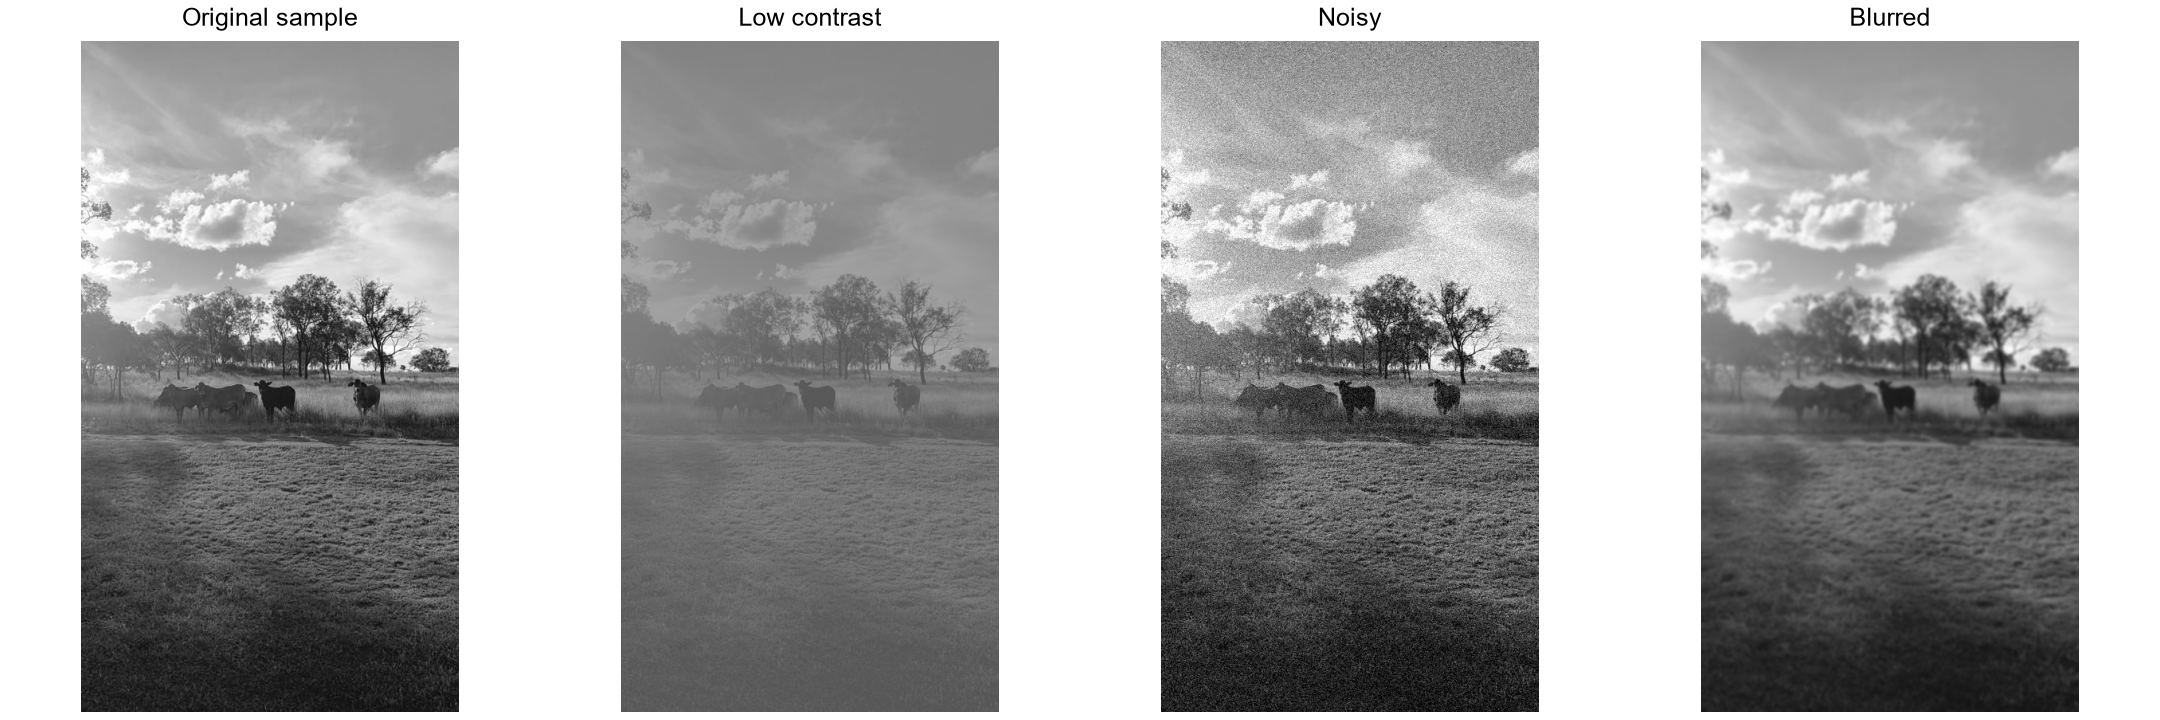
\includegraphics[width=\textwidth]{test_samples.png}
    \caption{Исходное изображение и сформированные тестовые варианты}
    \label{fig:samples}
\end{figure}

Рисунок~\ref{fig:samples} показывает исходный образец и три варианта для
проверки устойчивости методов. Малоконтрастная версия проверяет растяжение
диапазона и эквализацию; шумовая позволяет наблюдать ложные отклики
границ и лапласиана; размытие показывает влияние сглаживания на мелкие
детали и обнаружение границ. Варианты формируются программно, поэтому для
них не требуется отдельный набор исходных файлов.

\section{Проверка реализации}

Для проверки запущены три модульных теста:
\begin{enumerate}
    \item проверка min-max-преобразования, включая постоянное изображение;
    \item проверка наличия всех результатов обработки, типов данных и размеров
    выходных массивов;
    \item проверка набора тестовых вариантов и воспроизводимости генерации.
\end{enumerate}
Все три теста завершились успешно. Дополнительно проверена синтаксическая
корректность файлов программы и тестов.

\section{Вывод}

В работе создано приложение для полутоновых изображений, которое объединяет
min-max-контрастирование и эквализацию гистограммы с обнаружением точек,
линий и перепадов яркости. На тестовом изображении получены и сопоставлены
визуальные результаты, гистограммы и количественные характеристики.
Эквализация увеличила стандартное отклонение яркости выбранного изображения,
а детекторы Собеля и Кэнни сформировали карты границ с различной плотностью.
Воспроизводимые малоконтрастный, зашумленный и размытый варианты позволяют
проверять работу методов при изменении входных данных.

\section*{Список источников}
\addcontentsline{toc}{section}{Список источников}
\begin{enumerate}
    \item Gonzalez R.~C., Woods R.~E. Digital Image Processing. 4th ed.
    Pearson, 2018.
    \item OpenCV. Документация по обработке изображений:
    \texttt{https://docs.opencv.org/}.
    \item Методические указания к лабораторной работе № 2
    «Основы обработки цифровых изображений/сжатие изображений»,
    задание для варианта 4.
\end{enumerate}

\end{document}
